\documentclass[reqno,a4paper,12pt]{amsart}

\usepackage{amsmath,amssymb,amsthm,geometry,xcolor,soul,graphicx}
\usepackage{titlesec}
\usepackage{enumerate}
\usepackage{lipsum}
\usepackage{listings}
%\RequirePackage[most]{tcolorbox}
\usepackage{braket}
\allowdisplaybreaks[4] %align公式跨页
\usepackage{xeCJK}
\setCJKmainfont[AutoFakeBold = true]{Kai}
\geometry{left=0.7in, right=0.7in, top=1in, bottom=1in}

\renewcommand{\baselinestretch}{1.3}

\title{介观物理第二次作业}
\author{董建宇 ~~ 202328000807038}

\begin{document}

\maketitle
\titleformat{\section}[hang]{\small}{\thesection}{0.8em}{}{}
\titleformat{\subsection}[hang]{\small}{\thesubsection}{0.8em}{}{}

$Al_xGa_{1-x}/GaAs/Al_xGa_{1-x}As$量子阱的电子结构可以用一维有限深势阱模型来描述,势垒高度$V_b = 0.2eV$,势垒宽度$a=30nm$。

\begin{enumerate}[a)]

\item 假设势阱和势垒中导带电子的有效质量均为$m^* = 0.067m_0$,求解最低两个束缚态的能量本征值并给出相应的波函数;指出这两个能量本征值与同样宽度的无限深势阱的对应能级有多的区别,并定型解释其原因。

\begin{proof}
取$GaAs$左边界为坐标原点,向右为正方向,量子阱示意图如下:

\begin{center}
	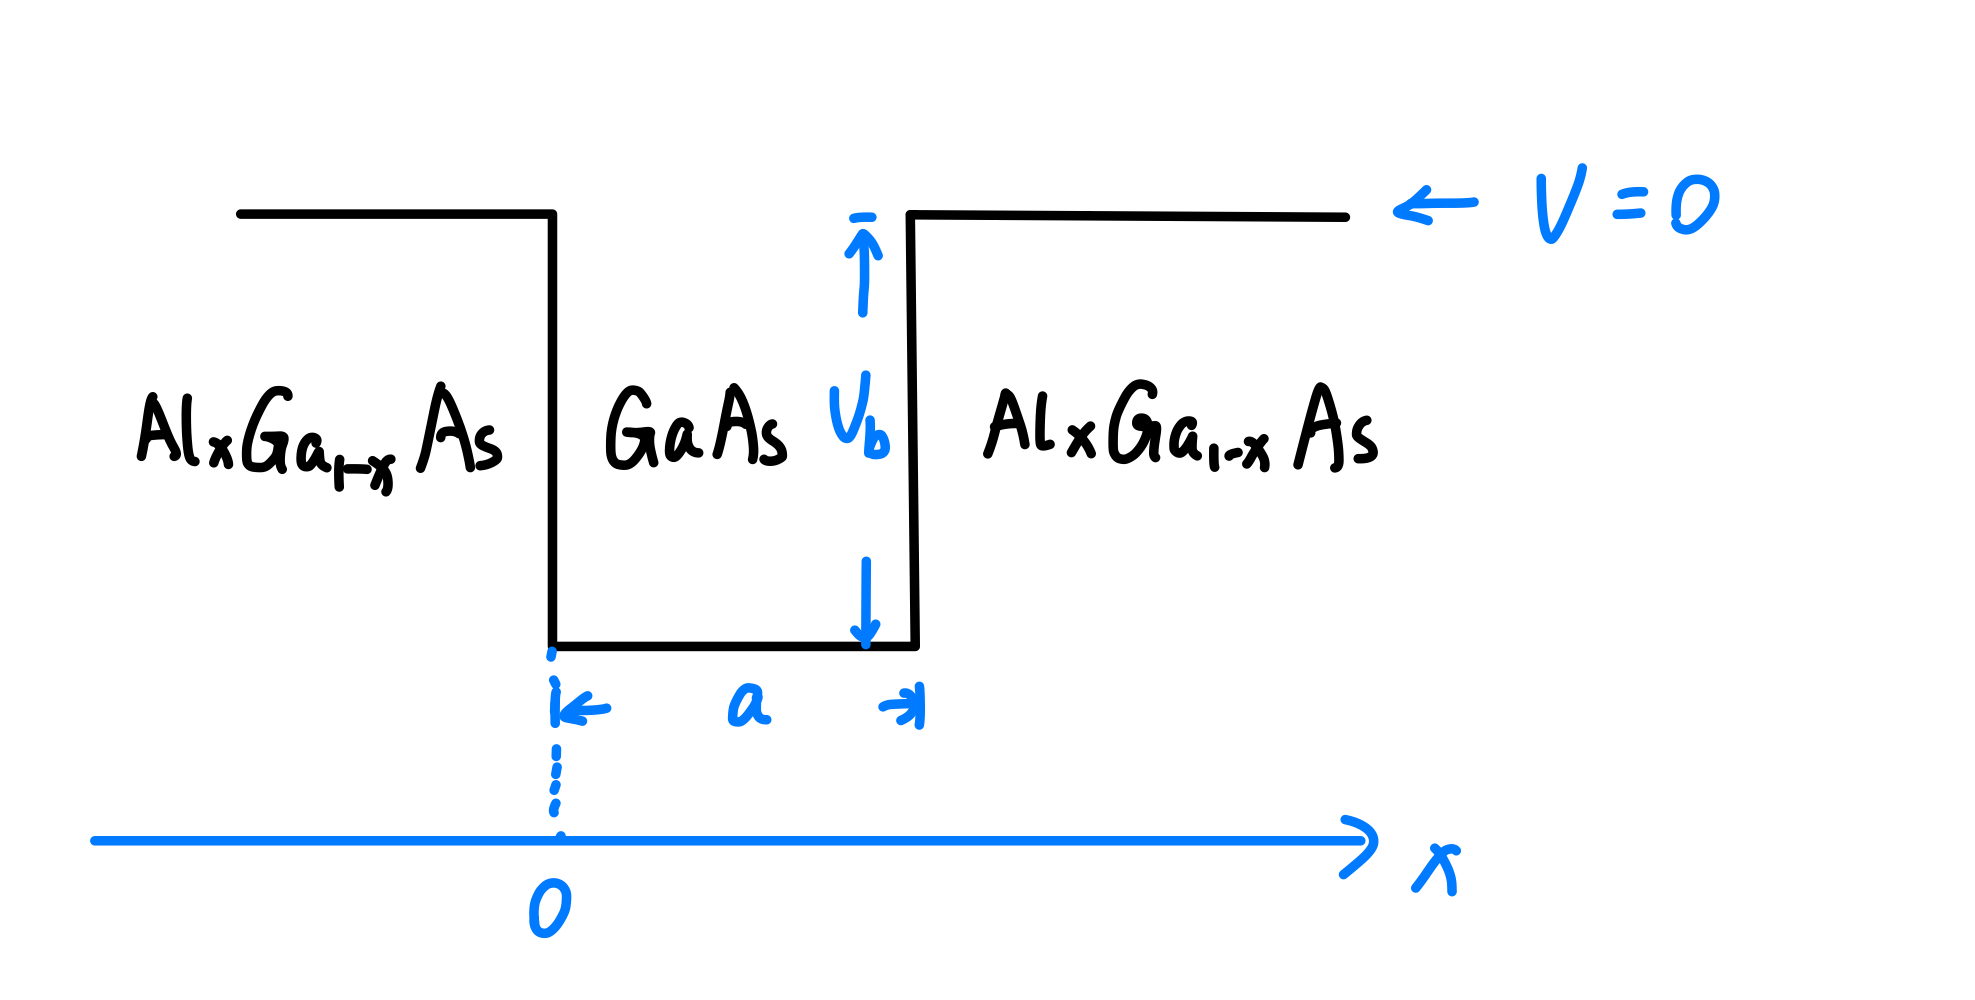
\includegraphics[scale = 0.18]{homework02.jpeg}
\end{center}

定态薛定谔方程可以写作:
\[
	\left( -\frac{\hbar^2}{2m^*} \frac{d^2}{dx^2} + V(x) \right) \psi_n(x) = E_n \psi_n(x).
\]

其中势能函数为:
\[
	V(x) = \left\{ \begin{aligned}
		&0, & &x\in (-\infty, 0) \cup (a, \infty); \\
		&-V_b, & &x \in (0,a).
	\end{aligned} \right.
\]

对于束缚态有:$-V_b < E_n < 0$,记:
\[
	k^2 = -\frac{2m^*E_n}{\hbar^2}; \ \ \kappa^2 = \frac{2m^*(V_b + E_n)}{\hbar^2}.
\]

注意到束缚态波函数满足:
\[
	\lim_{x\to \infty} \psi_n(x) = 0; \ \ \lim_{x\to -\infty} \psi_n(x) = 0.
\]

可以写出波函数通解为:
\[
	\psi_n(x) = \left\{ \begin{aligned}
		&Ae^{kx},& & x<0; \\
		&Ce^{i\kappa x} + De^{-i\kappa x},& & 0<x<a; \\
		&Be^{-kx},& & x>a.
	\end{aligned} \right.
\]

波函数的一阶导数为:
\[
	\psi_n(x)' = \frac{d\psi_n(x)}{dx} = \left\{ \begin{aligned}
		&Ake^{kx},& & x<0; \\
		&iC\kappa e^{i\kappa x} - iD\kappa e^{-i\kappa x},& & 0<x<a; \\
		&-Bke^{-kx},& & x>a.
	\end{aligned} \right.
\]

波函数以及波函数的一阶导数在$x=0$和$x=a$处连续,则有:
\begin{align*}
	&A = C + D \\
	&Be^{-ka} = Ce^{i\kappa a} + De^{-i\kappa a} \\
	&Ak = i(C-D)\kappa \\
	&-Bke^{-ka} = i\kappa (Ce^{i\kappa a} - De^{-i\kappa a})
\end{align*}

若此方程组有非平凡解,则系数行列式为0,即
\[
	\mathbf{det} \left( \begin{matrix}
		1 & 0 & -1 & -1 \\
		0 & e^{-ka} & -e^{i\kappa a} & -e^{-i\kappa a} \\
		k & 0 & -i\kappa & i\kappa \\
		0 & ke^{-ka} & i\kappa e^{i\kappa a} & -i\kappa e^{-i\kappa a}
	\end{matrix} \right) = 2ie^{-ka} (\kappa^2 \sin\kappa a - k^2\sin \kappa a - 2k\kappa \cos\kappa a) = 0.
\]

即
\[
	\tan \kappa a = \frac{2k\kappa}{\kappa^2 - k^2}.
\]

利用三角函数被角公式,可以得到:
\[
	\tan \kappa a = \frac{2\tan(\kappa a/2)}{1 - \tan^2(\kappa a/2)} = \frac{2(k/\kappa)}{1-(k/\kappa)^2}.
\]

可以解得:
\[
	\tan(\kappa a/2) = \frac{k}{\kappa}; \ \ \ \tan(\kappa a/2) = -\frac{\kappa}{k}.
\]

考虑第一种情况:$\tan(\kappa a/2) = \frac{k}{\kappa}$,注意到:
\[
	\frac{1}{\cos^2(\kappa a/2)} = 1 + \tan^2(\kappa a/2) = 1 + \frac{k^2}{\kappa^2} = \frac{k_0^2}{\kappa^2}.
\]

其中$k_0^2 = \kappa^2 + k^2 = \frac{2mV_0}{\hbar^2}$。则原方程化为:
\[
	\left\vert \cos\left( \frac{\kappa a}{2} \right) \right\vert = \frac{\kappa}{k_0}, \ \ \text{同时满足} \ \ \tan\left( \frac{\kappa a}{2} \right) > 0.
\]

考虑第二种情况:$\tan(\kappa a/2) = -\frac{\kappa}{k}$,注意到:
\[
	\frac{1}{\sin^2(\kappa a/2)} = 1 + \cot^2(\kappa a/2) = 1 + \frac{k^2}{\kappa^2} = \frac{k_0^2}{\kappa^2}.
\]

则原方程化为:
\[
	\left\vert \sin\left( \frac{\kappa a}{2} \right) \right\vert = \frac{\kappa}{k_0}, \ \ \text{同时满足} \ \ \tan\left( \frac{\kappa a}{2} \right) < 0.
\]

示意图如下:
\begin{center}
	\includegraphics[scale = 0.18]{homework02_02.jpeg}
\end{center}

其中红色曲线对应第一种情况,绿色曲线对应第二种情况,与蓝色直线的交点即为方程的解。

代入数据可得,能量最低的两个能量分别为:
\[
	E_1 = -0.195\text{eV}; \ \ E_2 = -0.180\text{eV}.
\]

对于无限深势阱,本征能量为:
\[
	E_n = \frac{n^2\pi^2\hbar^2}{2m^*a^2}, \ \ n = 1,2,\cdots.
\]

即:
\[
	E_{10} = 6.24\times 10^{-3}\text{eV}; \ \ E_{20} = 2.50\times 10^{-2}eV.
\]

若选取势阱底部为零势能面,有限深势阱下最低两个束缚态能量本征值分别为:
\[
	E_1' = 0.005eV; \ \ E_2' = 0.020eV.
\]

由于无限深势阱条件下,波函数仅被束缚在势阱内,势阱外严格为零;而有限高的势阱外波函数可以不为零。意味着无限深势阱条件下位置不确定度相对于有限深势阱更小,利用不确定性关系,意味着无限深势阱的栋梁不确定度更大,从而能量更高。
\end{proof}

\item 讨论势阱宽度$a$减小到多少时该量子阱只允许一个束缚态存在。

\begin{proof}
当量子阱中只允许一个束缚态存在时,从图中可以看出,要满足当$\sin(\kappa a/2)$第一次等于1,即$\kappa = \pi/a$时,$\kappa/k_0>1$,即有:
\[
	\frac{\pi}{a} > k_0 = \frac{\sqrt{2m^*V_b}}{\hbar}.
\]

代入数据可以计算:
\[
	a<5.30\text{nm}.
\]

即势阱宽度减小到$5.30\text{nm}$时,该量子阱只允许一个束缚态存在。
\end{proof}

\item 假设势垒区导带电子的有效质量变为$2m^*$,其余参数不变,讨论量子阱能及如何改变。

\begin{proof}
若电子有效质量变为$2m^*$,其余参数不变,带入$a)$中的方程可以计算得到最低两束缚态的能量本征值为:
\[
	E_1'' = -0.197\text{eV}; \ \ E_2'' = -0.189\text{eV}.
\]

即量子阱能级降低。
\end{proof}

\end{enumerate}




\end{document}